\section{Grundlagen}\label{sec:Grundlagen}

Die Abbildung \ref{fig:verschliesser} zeigt den neu entwickelten Dosenverschliesser. Die vier Falzrollen, die sich im unteren Teil der Maschine befinden, verschliessen die Dose. Die vier Falzwerkzeuge werden mit je einem Motor in die gewünschte Position gebracht. Auf einem Drehteller sind diese Motoren und die dazugehörigen Falzrollen angeordnet. Da dieser Drehteller rotiert, kann man die Kabel nicht direkt an die Motoren-Drives anschliessen. Dieses Problem wird mit einer Schleppkette (gelb markiert), die im oberen Teil der Maschine platziert ist, gelöst. Die Schleppkette führt die Kabel für die Energieversorgung und Datenkommunikation.

Der Nachteile dieser Lösung ist, dass die Schleppkette und dessen Halterung viel Platz benötigt. Zusätzlich wird sie sehr schnell verschmutzt und ist daher sehr wartungsintensiv. Aus diesen Gründen eignet sich das Konzept mit der Schleppkette nicht für eine Serienproduktion.

\begin{figure}[H]
	\centering
	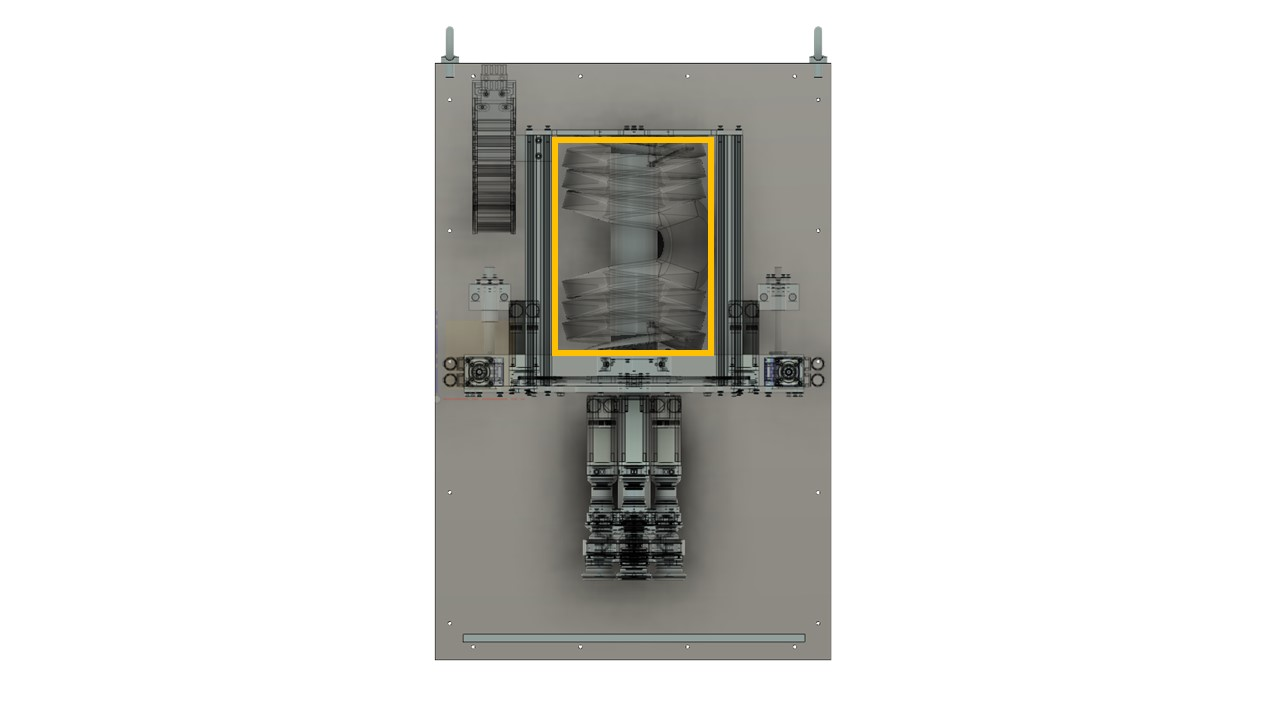
\includegraphics[width=0.5\linewidth]{verschliesser}
	\caption{Dossenverschliesser mit den Falzstationen und der Schleppkette}\label{fig:verschliesser}
\end{figure}

Der aktuelle Aufbau (Abbildung \ref{fig:gesamtkonzept}) besteht aus drei orangen Bauteilgruppen. Die blauen Blöcke kennzeichnen kabelgeführte Verbindung zwischen zwei Bauteilen. Um den Motor am Ende bedienen zu können, benötigt man ein Power-Kabel und ein Daten-Bus. Das aktuelle Konzept sieht vor, dass die Kabel mit einer Schleppkette zum Motoren-Drive geführt werden und von dort direkt auf den Motor. 

\begin{figure}[H]
	\centering
	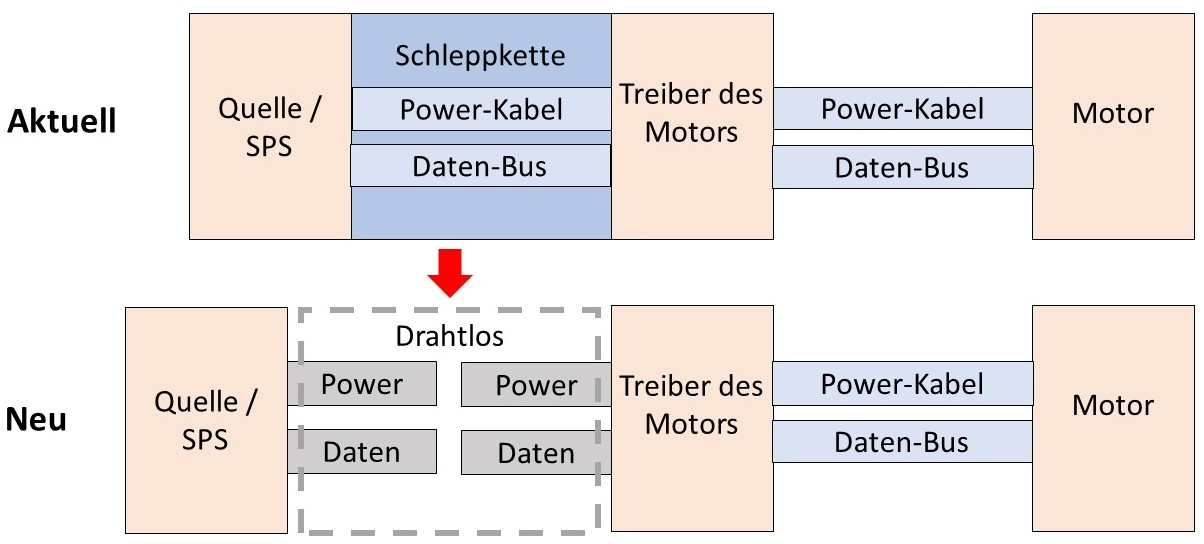
\includegraphics[width=0.9\linewidth]{gesamtkonzept}
	\caption{Aktuelles und neues Konzept der Energie- und Datenverbindung}\label{fig:gesamtkonzept}
\end{figure}

Da das aktuelle Konzept nicht die beste Lösung ist, soll die Verbindung zwischen der Quelle und dem Motor-Drive neu drahtlos realisiert werden. Im neuen Konzept wird das Power-Kabel durch die induktive Übertragung ersetzt und der Daten-Bus soll durch optische Übertragung gelöst werden. 

Die induktive Übertragung soll auf eine Leistung von mindestens $\SI{300}{W}/\SI{48}{V}$ ausgelegt werden, da dies die Leistung aller vier Motoren ist. Die optische Übertragung soll auf eine Datenübertragung mit einem VARAN Ethernet-Bus ausgelegt werden.

\subsection{Grundlagen zur Energieübertragung}
In diesem Unterkapitel werden die Grundlagen zur Energieübertragung erläutert. Das Kernstück der induktiven Übertragung ist ein Transformator. Dieser muss mit einer Schaltung angesteuert werden, damit sich das Magnetfeld ändert und Energie übertragen werden kann. Mittels diesen Grundlagen sollte die Theorie des Transformators und der Schaltung vermittelt werden.

\paragraph{Transformator}
Ein Transformator besteht im wesentlichen aus zwei eng gekoppelten Wicklungen oder Induktivitäten die meistens auf einem gemeinsamen Kern aus Eisen liegen. 

Der Kopplungsfaktor gibt Aufschluss darüber, wie stark die gegenseitige magnetische Beeinflussung zweier oder mehreren benachbarten Drahtschleifen durch Induktion infolge einer magnetischen Flussänderung ist. Die Schleifen, wie in Abbildung \ref{eq:kopplungsfaktor}, nennt man ideal gekoppelt, weil der magnetische Fluss der einen Drahtschleife vollständig von der anderen umschlossen wird. \cite{trafo}

\begin{figure}[H]
	\centering
	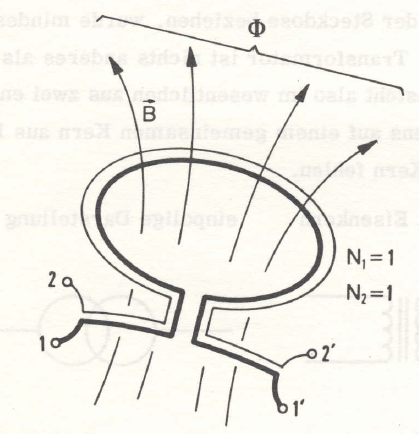
\includegraphics[width=0.4\linewidth]{kopplungsfaktor}
	\caption{Zwei ideal gekoppelte Einzelschleifen \cite{trafo}}\label{fig:kopplungsfaktor}
\end{figure}

Wenn sich in einer der beiden Schleifen der Strom ändert, induziert dieser sowohl in der eigenen als auch in der anderen Schleife dieselbe Spannung. Daher gilt Induktivität $ L_{1}$ = Induktivität $L_{2}$ = gesamte Gegeninduktivität $M$.
So lässt sich der Kopplungsfaktor $ k $ wie folgt definieren:\cite{trafo}
\begin{equation}
k=\frac{M}{\sqrt{L_{1}\cdot L_{2}}} = 1
\label{eq:kopplungsfaktor}
\end{equation}

In der Abbildung \ref{fig:trafo} ist ein ideal gekoppelter Transformator abgebildet. Die Ausgangsklemmen 2-2' sind offen was bedeutet, dass sich die Sekundärseite im Leerlauf befindet.\cite{trafo}
 
\begin{figure}[H]
	\centering
	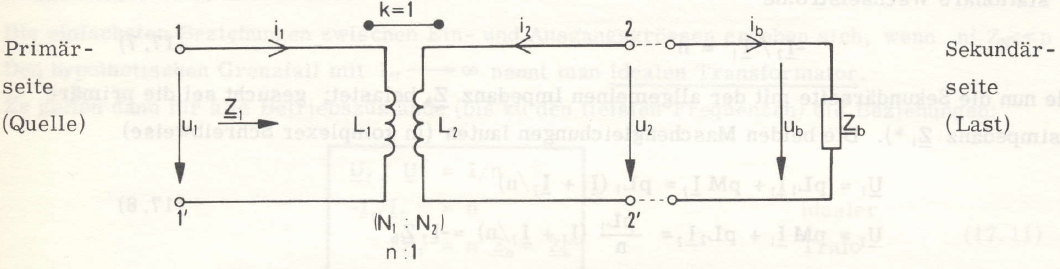
\includegraphics[width=1\linewidth]{grundlagen_trafo}
	\caption{Transformator mit ideal gekoppelten Spulen \cite{trafo}}\label{fig:trafo}
\end{figure}

In diesem Fall kann die Spannung $ u_{1} $ wie folgt berechnet werden.\cite{trafo}
\begin{equation}\label{eq:induktionsspannung}
u_{1}=L \cdot \frac{\mathrm{d} i_{L}}{\mathrm{d} t}
\end{equation}
Das Übersetzungsverhältnis ist beim idealen Transformator folgendermassen definiert.\cite{trafo}
\begin{equation}\label{eq:übertragung}
ü= \frac{N_{1}}{N_{2}} = \frac{U_{2}}{U_{1}}
\end{equation}

Lässt man nun die Voraussetzung der ideal gekopplten Spulen fallen, verhalten sich die induzierten Spannungen an zwei Induktivitäten nicht mehr wie die Windungszahlen. Die beiden Induktivitäten werden nun in einen ideal gekoppelten Teil und einen überhaupt nicht gekoppelten Teil aufgespaltenen. Der nicht gekoppelte Teil wird als Streuinduktivität bezeichnet. Sie hat Auswirkungen auf die Funktionsweise (Überspannung, Schwingungen nach Abschaltvorgängen) und Verluste von leistungselektronischen Schaltungen. Aus diesem Grund ist es wichtig einen möglichst idealen Kopplungsfaktor zu erreichen damit die Streuinduktivität klein ist.\cite{trafo}

\paragraph{Flyback-Converter}
Um eine Magnetfeldänderung zu erzeugen wird eine Schaltung benötigt. Die verwendete Schaltung wird Flyback-Converter oder auf Deutsch Eintakt-Sperrwandler genannt. Sie gehört zu den primär getakteten Wandlern. Die Eingangs- und Ausgangsseite sind galvanisch getrennt. Er wird in Schaltnetzteilen von kleiner bis mittlerer Leistung (ca. 500W), z.B. für PC-Netzteilen, Drucker und Fernsehgeräte eingesetzt. \cite{speerwandler} \cite{lea} 

Die Schaltung besteht aus wenigen Bauteilen. Dies sind ein Schalter, ein Speichertransformator, eine Diode und ein Kondensator. Der Schalter, z.B. ein MOSFET, wird mit einem konstanten Tastgrad und Frequenz gesteuert. \cite{bachelor}  

\begin{figure}[H]
\centering
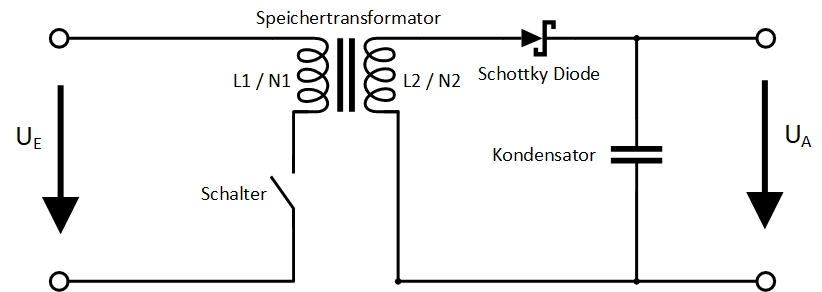
\includegraphics[width=1\linewidth]{flyback_schaltung}
\caption{Grundschaltung Flyback}\label{fig:flyback_schaltung}
\end{figure}

Wie man in Abbildung \ref{fig:flyback_schaltung} erkennen kann, beinhaltet die Schaltung einen Speichertransformator. Er dient zur dynamischen Energiespeicherung sowie für die Potenzialtrennung. Im Speichertransformator wird die gesamte übertragene Energie zwischen den einzelnen Zuständen im Magnetfeld zwischengespeichert. Aus diesem Grund benötigt er einen Luftspalt im Kern, da in diesem Teil die meiste magnetische Feldenergie gespeichert wird. Die beiden Wicklungen der Primär- und Sekundärseite müssen sehr gut magnetisch gekoppelt sein, damit die eingespeicherte Energie wieder abgegeben werden kann. Im Gegensatz dazu wird wegen der gleichzeitigen Leistungsaufnahme und -abgabe bei gewöhnlichen Transformatoren nur wenig Energie im Kern gespeichert.  \cite{speerwandler} \cite{lea} 

Der Flyback überträgt basierend auf diesem Prinzip seine Energie erst auf die Sekundärseite, wenn der Schalter auf der Primärseite geöffnet wird. Der Flyback ist prinzipiell kurzschlussfest, da die Diode auf der Sekundärseite sperrt, sobald der Schalter geschlossen wird. Die genauere Funktionsweise ist in der Tabelle \ref{tab:funktionsweise} aufgeführt. \cite{lea} 

\begin{table}[H]
	\centering
	\begin{tabular}{L{7cm}| L{7cm} }
		\multicolumn{1}{c|}{\textbf{Schalter geschlossen}}
		& \multicolumn{1}{c}{\textbf{Schalter geöffnet}} \\ \hline\hline
		$ \bullet $ Induktivität des Transformator lädt sich auf & $ \bullet $ Endmagnetisierung über die Sekundärwicklung \\ 
		$ \bullet $ Transformator ist im Leerlauf & $ \bullet $ Laden des Kondensators auf $ U_{A} $ \\ 
		$ \bullet $ Diode ist in Sperrrichtung &  \\ \hline
	\end{tabular}
	\caption{Funktionsweise des Flybacks \cite{lea} }\label{tab:funktionsweise}
\end{table}

\begin{figure}[H]
	\centering
	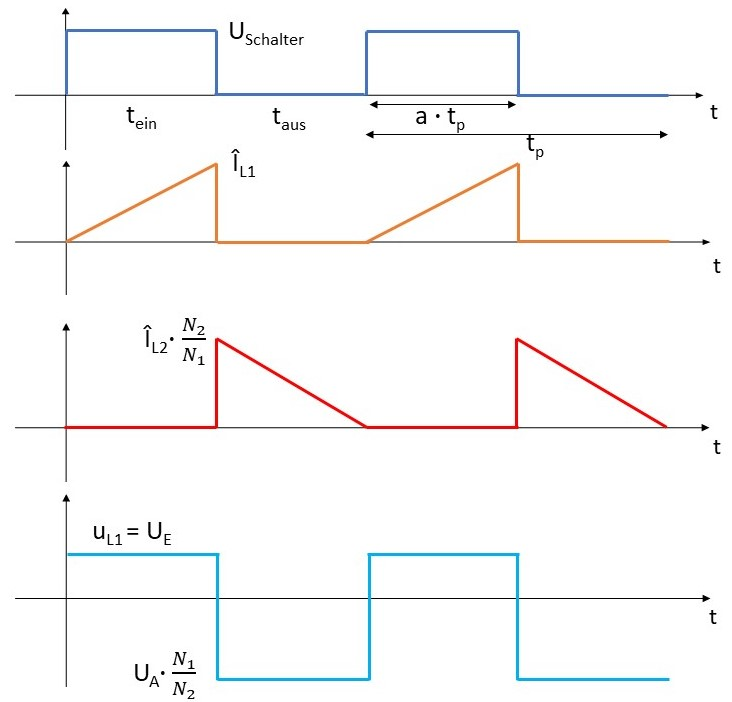
\includegraphics[width=0.9\linewidth]{kurven}
	\caption{Strom und Spannungsverlauf des Speichertrafos \cite{lea} }\label{fig:kurven}
\end{figure}

Die Abbildung \ref{fig:kurven} zeigt, dass während der Leitphase des MOSFET die Primärspannung $ u_{L1} $ des Trafos gleich der Eingangsspannung $ U_{E} $ ist. In dieser Zeit steigt der Strom $ i_{L1} $ linear an. Die Primärspannung wird mit der Formel \ref{eq:induktionsspannung} beschrieben. Die Primäspannung $ u_{L1} $ lässt sich in diesem Fall mit der Eingangsspannung $ U_{E} $  und $ \mathrm{d} t $ mit $ a \cdot T_{p} $ darstellen. Nun kann die Formel wie folgt nach $ \^{I}_{L1} $ umgeformt werden.\cite{lea} 

\begin{equation}\label{eq:strom}
\^{I}_{L1}=\frac{U_{E}}{L}\cdot a \cdot T_{p}
\end{equation}

Um die nachfolgenden Formeln zu vereinfachen, wird das Übersetzungsverhältnis $ ü $ aus der Formel \ref{eq:übertragung} eingesetzt. Die Primärspannung $ u_{L1} $ muss im stationärem Betrieb einen Mittelwert gleich Null haben. Ansonsten würde der Strom auf unermesslich hohe Werte ansteigen. Das Tastverhältnis hat den Kennbuchstaben $ a $. Daraus folgt $ 0= U_{E} \cdot a + ü \cdot (-U_{A}) \cdot (1-a) $. \cite{lea} Diese Gleichung lässt sich auch wie folgt schreiben:

\begin{equation}\label{eq:ausgangsspannung}
U_{A}= \frac{1}{ü} \cdot \frac{a}{1-a} \cdot U_{E}
\end{equation}

Die Energie, welche pro Periode übertragen wird, ist wie folgt zu berechnen:

\begin{equation}\label{eq:energie}
E= \frac{1}{2} \cdot L \cdot \^{I}_{p}\!^{2}
\end{equation}

Die übertragene Leistung hängt von der zwischengespeicherten Energie pro Periode und der Schaltfrequenz ab. Dies ergibt folgende Formel:

\begin{equation}\label{eq:Leistung}
P= f_{p} \cdot E = \frac{U_{2}\!^{2}}{R}
\end{equation}

\paragraph{Snubber}
Eine elektrische Schaltung, welche störende Spannungsspitzen neutralisieren soll, wird Snubber genannt. Solche Spannungsspitzen treten beim Schalten von induktiven Lasten auf, wenn der Strom abrupt unterbrochen wird. Dies ist auch beim Flyback der Fall, wenn der Schalter geöffnet wird. Aufgrund der Streuinduktivität des Speichertransformator steigt die Drain-Source-Spannung am MOSFET stark an. Diese Spannung kann den MOSFET beschädigen. Um diese Überspannung zu verhindern, gibt es verschiedene Möglichkeiten.\cite{teil_17} \cite{bachelor}

Ein Snubber zu dimensionieren, ist nicht ganz einfach den neben der Spannungsbegrenzung müssen noch weitere Probleme gelöste werden. Folgende Punkte müssen gelöst werden:
\begin{itemize}
	\item Spannungsbelastung des MOSFET auf ein aktzeptables Mass begrenzen
	\item Streuinduktivität möglichst zügig entladen, um den Wirkungsgrad hoch zu halten
	\item Schaltverluste dürfen nur minimal erhöht werden durch das Hinzufügen des Snubber-Glieds
	\item Auswirkungen auf das dynamische Verhalten des Netzteils zu vermeiden
\end{itemize}
Nachfolgend werden zwei Typologien vorgestellt.

\begin{figure}[H]
	\centering
	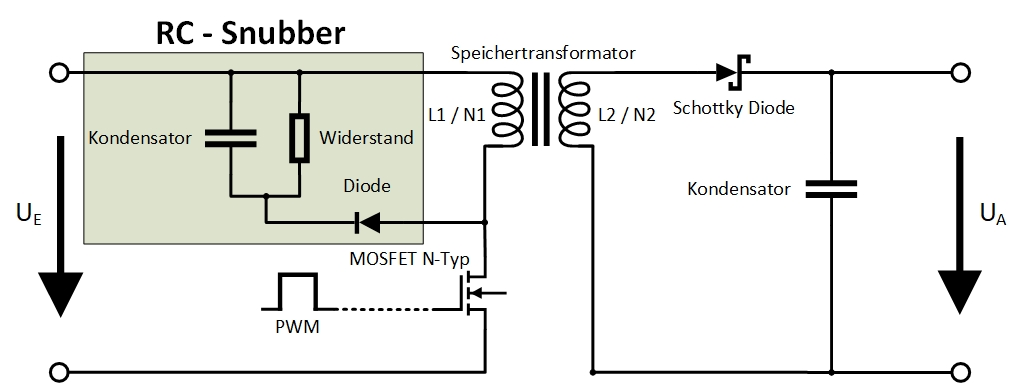
\includegraphics[width=0.9\linewidth]{Flyback_RC}
	\caption{Snubberschaltung mit RC-Glied}\label{fig:Flyback_RC}
\end{figure}

In der Abbildung \ref{fig:Flyback_RC} wird die Snubberschaltung mit einem Widerstand, einem Kondensator und einer Diode realisiert. Diese Schaltung basiert darauf, dass die überschüssige Energie aus der Streuinduktivität des Übertrags in den Snubber-Kondenstor geleitet wird. Die Differenz zwischen der Begrenzungs- und der Rest-Spannung ist gleich der Spannung über die Streuinduktivität. Die im Widerstand umgesetzte Verlustleistung und der Energiebetrag in der Streuinduktivität legen die Begrenzungsspannung dieser Schaltung fest. Ein kleiner Widerstand setzt die Begrenzungsspannung herab, jedoch entsteht eine höhere Verlustleistung.\cite{teil_17}  

Der Nachteil dieser Schaltung ist, je weiter die Begrenzungsspannung gesenkt wird, desto mehr Energie wird der Gesamtleistung entzogen. Daher entsteht ein schlechterer Wirkungsgrad.\cite{teil_17} 

\begin{figure}[H]
	\centering
	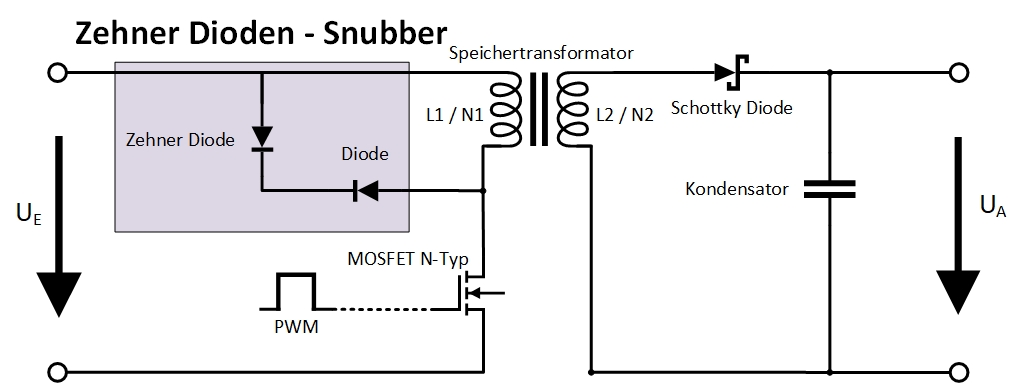
\includegraphics[width=0.9\linewidth]{Flyback_zehner}
	\caption{Snubberschaltung mit Zener- Diode}\label{fig:Flyback_zehner}
\end{figure}

Die zweite Snubber-Schaltung (Abbildung \ref{fig:Flyback_zehner}) besteht aus einer Zener-Diode und einer Diode. Die Drain-Spannung steigt nach dem Abschalten des MOSFET an, bis die Dioden leitend werden und die Streuinduktivität des Übertrags damit entladen. Die Differenz der reflektierten Ausgangspannung und der Zenerspannung bestimmt die Entladerate. Je schneller die Energie aus der Streuinduktivität abgebaut werden kann, desto besser ist der Wirkungsgrad. Die Werte der Dioden hängen von der zulässigen Spannungsbelastung des MOSFET ab. Nachdem die Streuinduktivität entladen ist, sollte die Z-Diode nicht mehr leiten. Aus diesem Grund sollte die Zenerspannung grösser als die reflektierte Ausgangsspannung sein. \cite{teil_54}

\subsection{Grundlagen zur Datenübertragung}
In diesem Unterkapitel werden einige Grundlagen zur Datenübertragung erläutert. Mittels dieser Grundlagen sollen die Eigenschaften des zu übertragenden Datenbussystems und Grundkenntnisse zu Photodioden und Empfängerschaltungen vermittelt werden. Es soll dem Leser als Basis für das Kapitel \textbf{\ref{sec:Daten} \nameref{sec:Daten}} dienen.

\paragraph{VARAN-Bus}
Der VARAN-Bus ist ein Echtzeit-Bussystem für die industrielle Automatisierung. Der Bus ist ein offener, herstellerunabhängiger Standard. Er verbindet Anlagen, Maschinen und Komponenten in der modernen Industrie. Das Bussystem arbeitet nach dem Manager-/Client-Prinzip. Weil der Manager die Kommunikation initialisiert, sind Paketkollisionen ausgeschlossen. Die Übertragungsschicht basiert auf dem Ethernet-Standard nach IEEE 802.3. Die verwendete 100TX-Standard-Ethernet-Technologie erlaubt eine maximale Übertragungsgeschwindigkeit von 100MBit pro Sekunde. \cite{varan-bus}

\paragraph{Ethernet}
Ethernet ermöglicht den kabelgebundenen Datenaustausch in Form von Datenframes zwischen Geräten in einem lokalen Netz. Dabei gibt es verschiedene Standards für unterschiedliche Übertragungsraten. Der 100Base-TX Standard (Fast Ethernet) des VARAN-Bus erlaubt eine maximale Datenrate von 100MBit/s. Statt der Manchesterkodierung, wie beim 10MBit/s-Ethernet, wird der effizientere 4B5B-Code eingesetzt. Dadurch wird eine Taktrückgewinnung aus dem Signal möglich. Durch eine zusätzliche MLT-3 Kodierung wird der Gleichspannungsanteil entfernt. \cite{ethernet}

\paragraph{4B5B Code:}
Der Leitungscode 4B5B bildet vier Nutzdatenbits auf fünf Codebits ab. Dadurch erhöht sich die codierte Bitrate um 25\%. Beim verwendeten Ethernet-Standard beträgt die codierte Symbolrate somit 125MBit/s. Bei der Abbildung auf fünf Codebits werden lange '0'-oder '1'-Folgen vermieden. Dadurch wird die Taktrückgewinnung aus dem Signal verbessert. \cite{4b5b}

\paragraph{MLT-3 Code:}
Multilevel Transmission Encoding (MLT-3) ist ein Leitungscode mit drei Spannungspegeln. Diese werden mit den Symbolen (+,\ 0,\ -) bezeichnet. Bei einer logischen '1' ändert sich der Spannungspegel nach der fixen Folge [0,\ +,\ 0,\ -]. Wird eine logische '0' übertragen, ändert sich der Zustand der Leitung nicht. Abbildung \ref{fig:MLT3code} zeigt eine beliebige Datenfolge mit der dazugehörigen MLT-3 Codierung. \cite{MLT-3}
\begin{figure}[h]
\centering
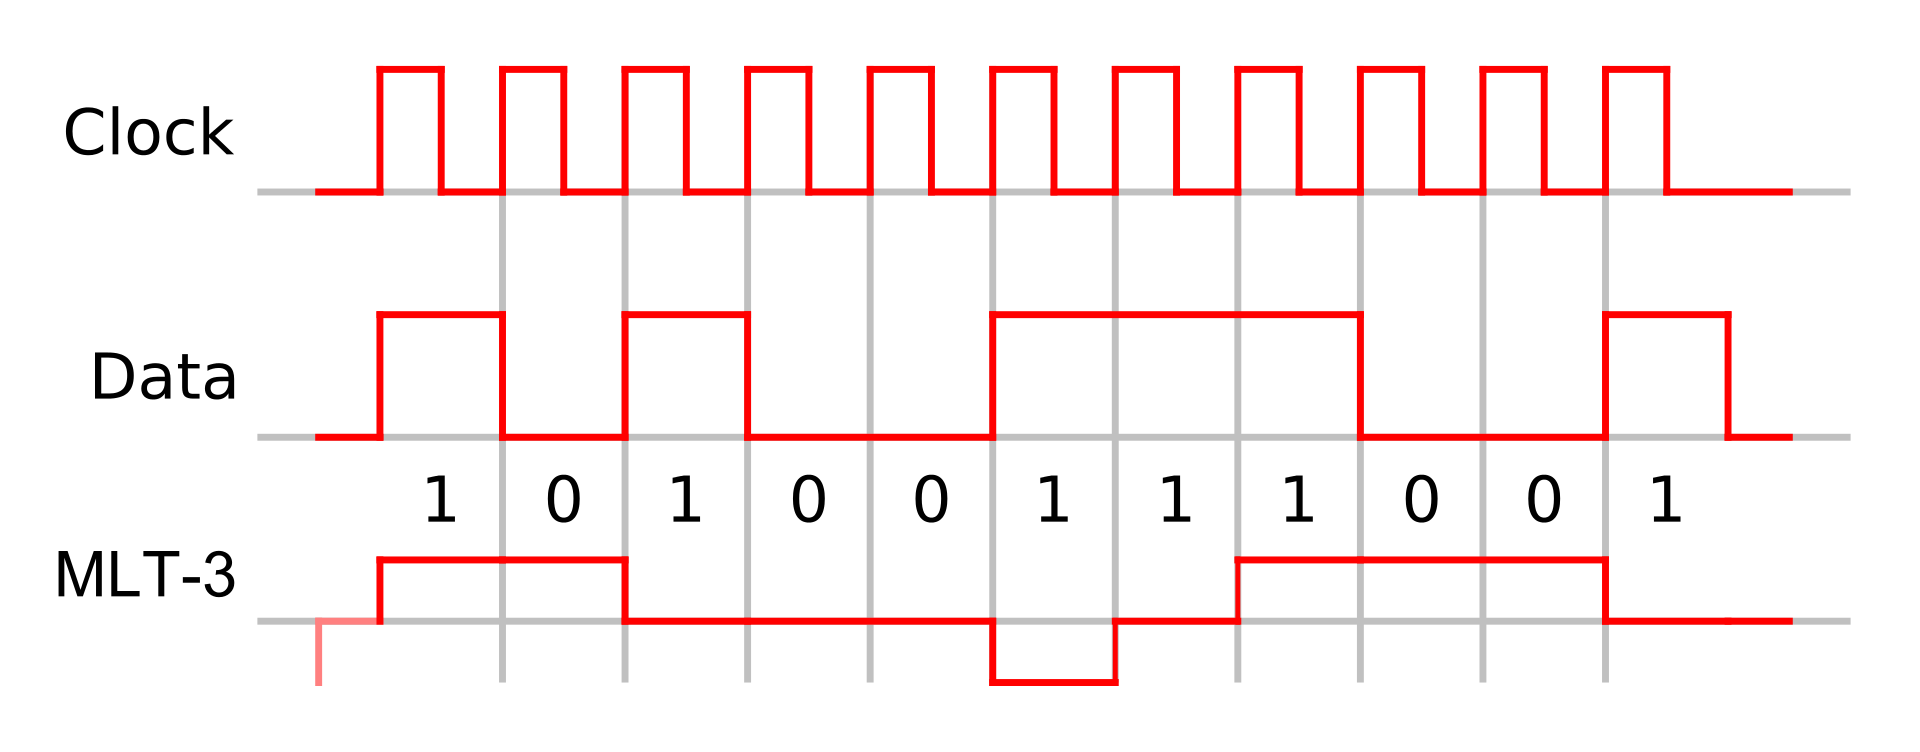
\includegraphics[width=0.8\linewidth]{MLT3encoding.png}
\caption{MLT-3 codierte Datenfolge \cite{MLT-3Bild}}\label{fig:MLT3code}
\end{figure}

In einer Übertragungsschwingung werden 4 Bit übertragen. Damit reduziert sich die eigentliche Übertragungsfrequenz auf einen Viertel der Symbolrate. Die maximale Übertragungsfrequenz auf der Leitung beträgt demnach: 
\begin{equation}\label{eq:MLT3}
f_{max}=\frac{Symbolrate}{4 Bit}=\frac{125Mbit/s}{4 Bit}=31.25 MHz
\end{equation}
Um die Datenrate von \SI{100}{MBit/s} zu erreichen, dürften also \SI{31.25}{MHz} ausreichen.

\paragraph{Messung VARAN-Bus}
Abbildung \ref{fig:Messung_Varan} zeigt den VARAN-Bus während einer Übertragung, gemessen mit einer Stromsonde.
\begin{figure}[H]
	\centering
	\includegraphics[width=0.5\linewidth]{Messung_Varan.png}
	\caption{VARAN-Bus Signal im Betrieb}\label{fig:Messung_Varan}
\end{figure}
Die höchste aufgetretene Frequenz beträgt: $\frac{1}{\SI{41}{ns}}\approx \SI{24.4}{MHz}$. Es ist trotzdem sinnvoll, die Schaltung auf die berechneten \SI{31.25}{MHz} auszulegen. So hat man einen gewissen Spielraum.

\paragraph{Photodioden-Verstärker}
Photodioden sind Halbleiter-Dioden, die auftreffende Photonen in einen elektrischen Strom umwandeln. Abbildung \ref{fig:Kenn_Photodiode} zeigt die typische U-I-Kennlinie einer Photodiode.
\begin{figure}[h]
	\centering
	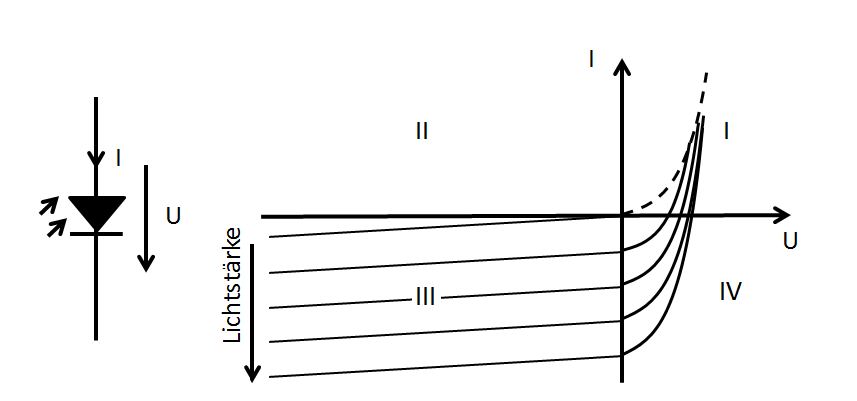
\includegraphics[width=0.8\linewidth]{Kennlinie_Photodiode.png}
	\caption{typische Kennlinie einer Photodiode \cite{schleuniger}}\label{fig:Kenn_Photodiode}
\end{figure}
Da im dritten Quadranten ein linearer Zusammenhang zwischen Lichtstärke und Photostrom erkennbar ist, eignet sich dieser Bereich für Sensoranwendungen und in unserem Fall auch Signalübertragungen.
Eine reale Photodiode besteht aus einer idealen Diode und einer parallel geschalteten Stromquelle. Der Strom ist abhängig von der Lichtstärke. Ein hochohmiger Widerstand stellt den Dunkelstrom der Photodiode dar. Die parasitäre Kapazität hängt primär von der Geometrie der Diode ab.
 \begin{figure}[H]
 	\centering
 	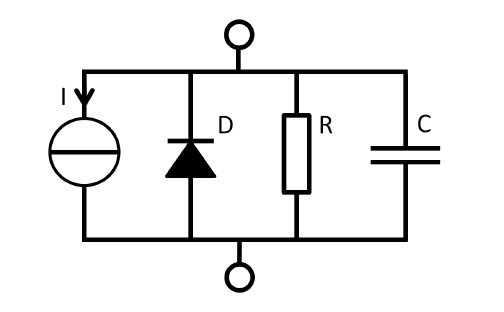
\includegraphics[width=0.8\linewidth]{Ersatzschaltbild_Photodiode.png}
 	\caption{Ersatzschaltbild einer Photodiode \cite{schleuniger}}\label{fig:Ersatz_Photodiode}
 \end{figure}
Für eine richtige Dimensionierung einer Schaltung, sind diese Parameter des Ersatzschaltbildes unbedingt zu beachten. Vor allem bei höheren Frequenzen hat die parasitäre Kapazität einen starken Einfluss. Der Widerstand ist normalerweise im Mega- oder Gigaohm-Bereich und kann vernachlässigt werden. \newline

Der Photostrom liegt meist im Nanoampere-Bereich und muss entsprechend verstärkt werden. Mit Hilfe eines Photodioden-Verstärkers wird der Photostrom in eine proportionale Spannung gewandelt. Meist werden dafür Transimpedanzverstärkerschaltungen eingesetzt.
\begin{figure}[h]
	\centering
	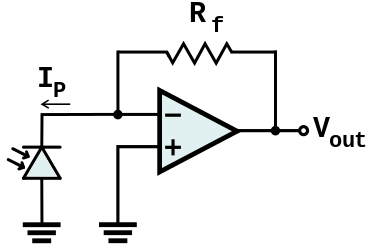
\includegraphics[width=0.5\linewidth]{Photo_Amp.png}
	\caption{Transimpedanzverstärker \cite{PhotoAmp}}\label{fig:Photo_Amp}
\end{figure}

Da die Eingänge des Verstärkers hochimpedant sind, fliesst der Photostrom $ I_{p} $ nur durch den Rückkopplungswiderstand $ R_{f} $. Am Ausgang des Verstärkers stellt sich eine positive Spannung proportional zum Strom $ I_{p} $ ein. Die Ausgangsspannung beträgt:
\begin{equation}\label{eq:Vout_Photo}
V_{out}=R_{f} \cdot I_{p}
\end{equation}

Aus der Formel \ref{eq:Vout_Photo} ist leicht ersichtlich, dass $ R_{f} $ dem Verstärkungsfaktor der Transimpedanzverstärkerschaltung entspricht.

Die Bandbreite eines Photodiodenverstärkers ist begrenzt und hängt vom Gain-Bandwidth Product $GBWP$ des Operationsverstärkers, dem Rückkopplungswiderstand $ R_{f} $ und den parasitären Kapazitäten von Operationsverstärker $ C_{opamp} $ und Photodiode $ C_{photo} $ ab. Mit folgender Formel \ref{eq:Bandwidth} kann die Bandbreite berechnet werden:

\begin{equation}\label{eq:Bandwidth}
B=\sqrt{\frac{GBWP}{2\pi\cdot R_{f}\cdot (C_{opamp}+C_{photo})}}
\end{equation}

Wie man in der Formel erkennen kann, begrenzt unter anderem die Kapazität $ C_{photo} $ der Photodiode die Bandbreite der Schaltung. Durch Anlegen einer negativen Biasspannung an der Anode der Photodiode, kann $ C_{photo} $ reduziert werden.

Für eine Anwendung mit hoher Bandbreite, wie in dieser Arbeit verlangt, ist also ein Operationsverstärker mit hohem Gain-Bandwidth Product $GBWP$ und kleiner Eingangskapazität $ C_{opamp} $ gewünscht. Ausserdem wird idealerweise eine Photodiode mit kleiner parasitärer Kapazität $ C_{photo} $ verwendet und diese zusätzlich durch Anlegen einer negativen Biasspannung reduziert. \cite{schleuniger} \cite{design_photo}
